\documentclass[11pt,a4paper,titlepage]{article}
\usepackage[a4paper]{geometry}
\usepackage[utf8]{inputenc}
\usepackage[english]{babel}
\usepackage{lipsum}

\usepackage{amsmath, amssymb, amsfonts, amsthm, mathtools}
% mathtools for: Aboxed (put box on last equation in align envirenment)
\usepackage{microtype} %improves the spacing between words and letters

\usepackage{lipsum}
\usepackage{threeparttable}
\usepackage{tabularx}
\usepackage{multirow}
\usepackage{booktabs}
\newcommand{\tabitem}{~~\llap{\textbullet}~~}
\usepackage{graphicx}
\graphicspath{ {./figures/} {./eps/}}
\usepackage{epsfig}
\usepackage{epstopdf}
\usepackage{verbatim}
\usepackage{textcomp}
\usepackage{tikz}
\usetikzlibrary{shapes,arrows}

%%%%%%%%%%%%%%%%%%%%%%%%%%%%%%%%%%%%%%%%%%%%%%%%%%
%% COLOR DEFINITIONS
%%%%%%%%%%%%%%%%%%%%%%%%%%%%%%%%%%%%%%%%%%%%%%%%%%
 % Enabling mixing colors and color's call by 'svgnames'
%%%%%%%%%%%%%%%%%%%%%%%%%%%%%%%%%%%%%%%%%%%%%%%%%%
\definecolor{MyColor1}{rgb}{0.2,0.4,0.6} %mix personal color
\newcommand{\textb}{\color{Black} \usefont{OT1}{lmss}{m}{n}}
\newcommand{\blue}{\color{MyColor1} \usefont{OT1}{lmss}{m}{n}}
\newcommand{\blueb}{\color{MyColor1} \usefont{OT1}{lmss}{b}{n}}
\newcommand{\red}{\color{LightCoral} \usefont{OT1}{lmss}{m}{n}}
\newcommand{\green}{\color{Turquoise} \usefont{OT1}{lmss}{m}{n}}
%%%%%%%%%%%%%%%%%%%%%%%%%%%%%%%%%%%%%%%%%%%%%%%%%%


%%%%%%%%%%%%%%%%%%%%%%%%%%%%%%%%%%%%%%%%%%%%%%%%%%
%% FONTS AND COLORS
%%%%%%%%%%%%%%%%%%%%%%%%%%%%%%%%%%%%%%%%%%%%%%%%%%
%    SECTIONS
%%%%%%%%%%%%%%%%%%%%%%%%%%%%%%%%%%%%%%%%%%%%%%%%%%
\usepackage{titlesec}
\usepackage{sectsty}
%%%%%%%%%%%%%%%%%%%%%%%%
%set section/subsections HEADINGS font and color
\sectionfont{\color{MyColor1}}  % sets colour of sections
\subsectionfont{\color{MyColor1}}  % sets colour of sections

%set section enumerator to arabic number (see footnotes markings alternatives)
\renewcommand\thesection{\arabic{section}.} %define sections numbering
\renewcommand\thesubsection{\thesection\arabic{subsection}} %subsec.num.

%define new section style
\newcommand{\mysection}{
\titleformat{\section} [runin] {\usefont{OT1}{lmss}{b}{n}\color{MyColor1}}
{\thesection} {3pt} {} }

%%%%%%%%%%%%%%%%%%%%%%%%%%%%%%%%%%%%%%%%%%%%%%%%%%
%		CAPTIONS
%%%%%%%%%%%%%%%%%%%%%%%%%%%%%%%%%%%%%%%%%%%%%%%%%%
\usepackage{caption}
\usepackage{subcaption}
%%%%%%%%%%%%%%%%%%%%%%%%
\captionsetup[figure]{labelfont={color=MyColor1}}

%%%%%%%%%%%%%%%%%%%%%%%%%%%%%%%%%%%%%%%%%%%%%%%%%%
%		!!!EQUATION (ARRAY) --> USING ALIGN INSTEAD
%%%%%%%%%%%%%%%%%%%%%%%%%%%%%%%%%%%%%%%%%%%%%%%%%%
%using amsmath package to redefine eq. numeration (1.1, 1.2, ...)
%%%%%%%%%%%%%%%%%%%%%%%%
\renewcommand{\theequation}{\thesection\arabic{equation}}

%set box background to grey in align environment
\usepackage{etoolbox}% http://ctan.org/pkg/etoolbox
\makeatletter
\patchcmd{\@Aboxed}{\boxed{#1#2}}{\colorbox{black!15}{$#1#2$}}{}{}%
\patchcmd{\@boxed}{\boxed{#1#2}}{\colorbox{black!15}{$#1#2$}}{}{}%
\makeatother
%%%%%%%%%%%%%%%%%%%%%%%%%%%%%%%%%%%%%%%%%%%%%%%%%%



\makeatletter
\let\reftagform@=\tagform@
\def\tagform@#1{\maketag@@@{(\ignorespaces\textcolor{red}{#1}\unskip\@@italiccorr)}}
\renewcommand{\eqref}[1]{\textup{\reftagform@{\ref{#1}}}}
\makeatother
\usepackage[hidelinks]{hyperref}

%% LISTS CONFIGURATION %%
\usepackage{enumitem}
\setlist[enumerate,1]{start=0}
\renewcommand{\labelenumii}{\theenumii}
\renewcommand{\theenumii}{\theenumi.\arabic{enumii}.}

%%%%%%%%%%%%%%%%%%%%%%%%%%%%%%%%%%%%%%%%%%%%%%%%%%
%% PREPARE TITLE
%%%%%%%%%%%%%%%%%%%%%%%%%%%%%%%%%%%%%%%%%%%%%%%%%%
\title{\blue Satellite Communications \\
\blueb Satellite system to provide communication services to polar regions in Europe and Russia}
\author{Ana Reviejo Jiménez \\ Marta Munilla Díez\\ Oscar Pla Terrada\\ Davide Peron\\ Cristina Gava\\ Javier Garcia Camin}
\date{\today}
%%%%%%%%%%%%%%%%%%%%%%%%%%%%%%%%%%%%%%%%%%%%%%%%%%

\begin{document}
\maketitle

\tableofcontents
\clearpage

\section{Problem Description} \label{sec:problem_description}
	\begin{figure}
	\centering
	\begin{minipage}{0.45\textwidth}
		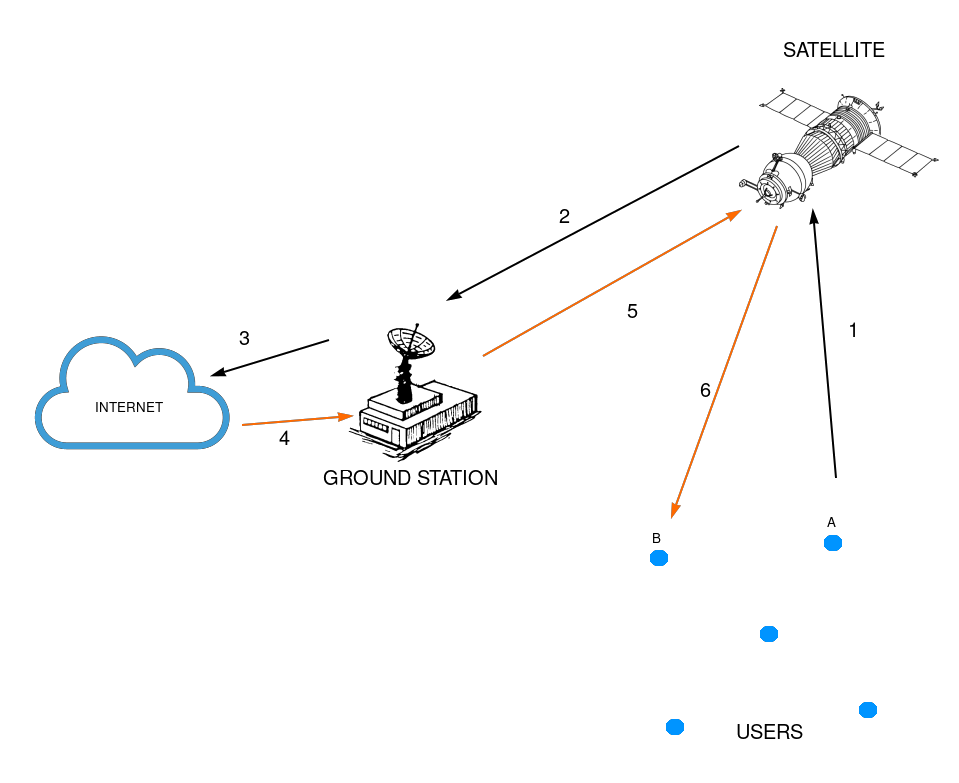
\includegraphics[width=\textwidth]{figures/System_topology_noBG.png}
		\caption{Scheme of the topology of the system.}
		\label{fig:topology}
	\end{minipage}\hspace{0.5cm}
	\begin{minipage}{0.45\textwidth}
		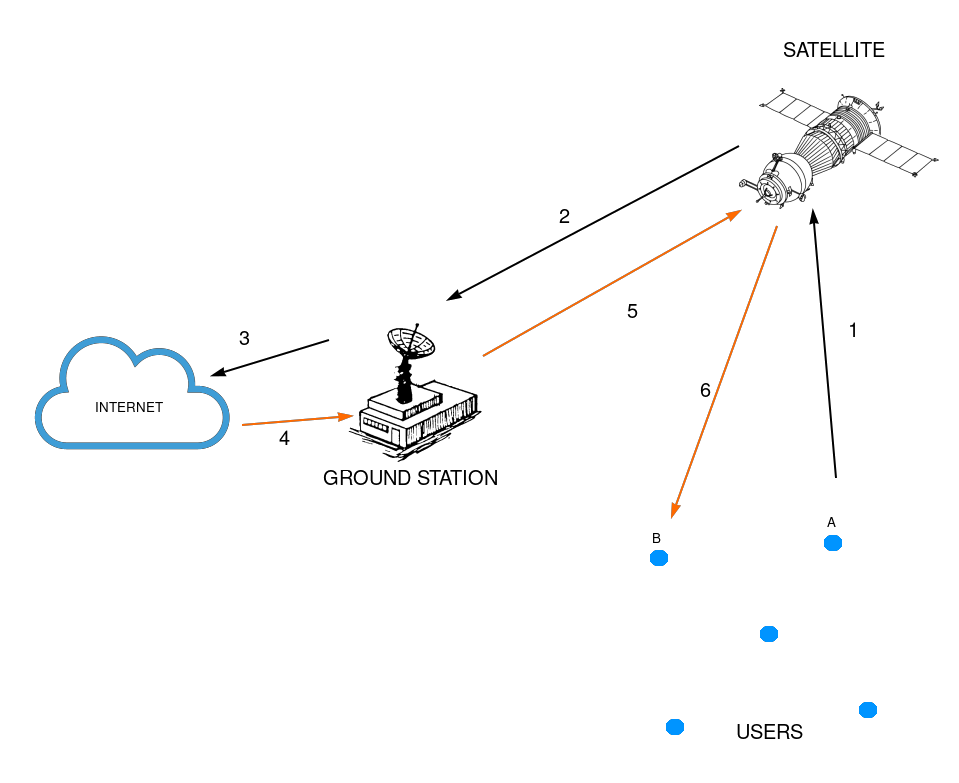
\includegraphics[width=\textwidth]{figures/System_topology_noBG.png}
		\caption{Typical communication path between an user A and an user B.}
		\label{fig:communication}
	\end{minipage}
\end{figure}

This project results from the necessity of having a good broadband coverage of polar
areas and the land areas of Northern Europe and Russia: this means the coverage of
latitudes over the 60 deg.

The subjects interested in this kind of communication are
mostly industries involved in economic sector: they need a reliable communication system able to provide a service of 50 Mbps in download and 5 Mbps in upload.


The aim is to project a system able to provide a continuous, reliable and feasible communication service, maximizing the number of users allowed to access it over $60^\circ$
latitudes and minimizing the costs. To do that, services in narrowband communication using LEO satellites are not useful, since the broadband communication required is not feasible with this technology.

A simple representation of the system to be built is shown in \autoref{fig:topology} and a communication between two users is in \autoref{fig:communication}.

Typically, if a user A has to communicate with user B, it sends his packets to the satellite, with the recipient address in the header.
The satellite receives the packets and forwards them to the Ground Station that sends them to the proper application (Skype, Hangout, ...).
These packets are sent from the application to the Ground Station, that forwards them, through the satellite, to the recipient B.


\section{Simulator and Orbits} \label{sec:orbit}
	\subsection{Simulator Architecture}
		\lipsum[2]
	\subsection{Orbit selection}
		The parameters of the orbits analysed in the simulator are presented in \autoref{tab:orbits}.

\begin{table}
	\centering
	\begin{tabular}{ccc}
	\toprule
	& Tundra & Molniya\\
	\midrule
	Orbital Period (s)     & 86400   & 43200\\
	Eccentricity        & 0.25   & 0.71\\
	Semi-major axis (km) & 42164 & 26556\\
	Inclination (deg)      & 63.4 & 63.4\\
	\bottomrule
	\end{tabular}
	\caption{Parameters of the considerated orbits}
	\label{tab:orbits}
\end{table}


\section{Payload and Space Segment}
		\lipsum[1]
	\subsection{Communication Module}
		\lipsum[1]
	\subsection{Payload}
		% Definition of blocks:
\tikzset{%
  block/.style    = {draw, thick, rectangle, minimum height = 3em,
    minimum width = 3em},
	rect/.style    = {draw, thick, rectangle, minimum height = 3em,
	    minimum width = 1.5em},
	mux/.style    = {draw, thick, rectangle, minimum height = 7em,
			minimum width = 2.5em, align=left},
	triang/.style    = {draw, thick, isosceles triangle, minimum height = 3em, minimum width = 1.5em, align=left},
  mult/.style      = {draw, circle, node distance = 2.7cm},
  ghost/.style    = {coordinate}, % Input
  output/.style   = {coordinate} % Output
}
% Defining string as labels of certain blocks.
\newcommand{\mult}{\Large$\times$}
\newcommand{\inte}{$\displaystyle \int$}
\newcommand{\derv}{\huge$\frac{d}{dt}$}

\begin{tikzpicture}[auto, thick, node distance=2cm, >=triangle 45]
\draw
	% Drawing the blocks of first filter :
	node at (0,0)[right=-3mm, , label={below:(0)}]{\Large \textopenbullet}
	node [ghost, name=input1] {}
	% node [sum, right of=input1] (suma1) {\suma}
	node [rect, right of=input1, label={below:(1)}] (pol_sep) {}
  node [triang, right of=pol_sep, label={below:(2)}] (lna) {LNA}
  node [mult, right of=lna, label={D/C}, label={below:(3)}] (dlc) {\mult}
	node [triang, right of=dlc, label={below:(4)}] (ifa) {IF \\ amp}
	node [mult, right of=ifa, label={U/C}, label={below:(5)}] (ulc) {\mult}
	node [triang, right of=ulc, label={below:(6)}] (hpa) {HPA}
	node [triang, right of=hpa, label={below:(7)}] (bpf) {}
	node [mux, right of=bpf] (imux) {I \\M \\U \\ X}
	node at (19,1.5)[right=-3mm, name = ch1, label={left:$ch_1$}]{\Large \textopenbullet}
	node at (19,1)[right=-3mm, name = ch2]{}
	node at (19,0.5)[right=-3mm, name = ch3]{}
	node at (19,0)[right=-3mm, name = ch4]{}
	node at (19,-1.5)[right=-3mm, name = chN, , label={left:$ch_N$}]{}
	node [triang, right of=ch1, label={below:(8)}] (ca) {}
	node [block, right of=ca, label={below:(9)}] (alc) {ALC}
	node [triang, right of=alc, label={below:(10)}] (outamp) {}
	node [mux, right of=imux, node distance = 10cm] (omux) {O \\M \\U \\ X}
	node [triang, right of=omux, label={below:(11)}] (bpf2) {}
	node at (32,0)[right=-3mm, name = outantenna, label={below:(12)}]{\Large \textopenbullet};
    % Joining blocks.
    % Commands \draw with options like [->] must be written individually
	\draw[-](input1) -- node {}(pol_sep);
	\draw[-](pol_sep) -- node {} (lna);
	\draw[-](lna) -- node {$f_D$} (dlc);
	\draw[-](dlc) -- node {$f_{IF}$} (ifa);
	\draw[-](ifa) -- node {$f_{IF}$} (ulc);
	\draw[-](ulc) -- node {$f_u$} (hpa);
	% \draw[-](rx) -- node {} (bpf);
	\draw[-](hpa) -- node {} (bpf);
	\draw[-](bpf) -- node {} (imux);
	\draw[-](imux) -- node {} (ch1);
	\draw[-](imux) -- node {} (ch2);
	\draw[dashed](imux) -- node {} (ch3);
	\draw[dashed](imux) -- node {} (ch4);
	\draw[-](imux) -- node {} (chN);
	\draw[-](ch1) -- node {} (ca);
	\draw[-](ca) -- node {} (alc);
	\draw[-](alc) -- node {} (outamp);
	\draw[-](outamp) -- node {} (omux);
	\draw[-](omux) -- node {} (bpf2);
	\draw[-](bpf2) -- node {} (outantenna);

% 	% Boxing and labelling
	\draw [color=gray, dashed, label={Receiver Block}](1,-1.5) rectangle (14.5,1.5);
	\node at (6.5,1.5) [above=5mm, right=0mm] {\textsc{Receiver Block}};

	\draw [color=gray, dashed, label={Receiver Block}](14.8,2.5) rectangle (31,-2.5);
	\node at (21.5,2.5) [above=5mm, right=0mm] {\textsc{Repeater Block}};
	\draw [color=gray,thick](-0.5,-9) rectangle (12.5,-5);
	\node at (-0.5,-9) [below=5mm, right=0mm] {\textsc{second-order noise shaper}};
\end{tikzpicture}
		\subsubsection{Receiver Block}
			\lipsum[1]
		\subsubsection{Repeater Block}
			\lipsum[1]
	\subsection{Power Budget}
		\subsubsection{Required Power}
			\lipsum[1]
		\subsubsection{Solar Panels specifications}
			\lipsum[1]
	\subsection{Weight Estimation}
		\lipsum[1]

\section{Ground Segment}
	\lipsum[1]
	\subsection{Ground Station coordinates}
		\lipsum[1]
	\subsection{Ground Station requirements}
		\lipsum[1]
	\subsection{User requirements}

\section{Link Budget}
	\subsection{Parameters setting and estimation}
		\subsubsection{Antenna Parameters}
		\subsubsection{Effective Isotropic Radiated Power(EIRP)}
		\subsubsection{Losses}
	\subsection{Uplink}
	\subsection{Downlink}
	\subsection{Overall Link Budget}
\lipsum[1]

\section{Cost Estimation}
	\subsection{Spacecraft cost}
	\subsection{Launch cost}
	\lipsum[1]

\section{Final considerations and conclusions}
	\lipsum[1]

\end{document}
